\documentclass[1p]{elsarticle_modified}
%\bibliographystyle{elsarticle-num}

%\usepackage[colorlinks]{hyperref}
%\usepackage{abbrmath_seonhwa} %\Abb, \Ascr, \Acal ,\Abf, \Afrak
\usepackage{amsfonts}
\usepackage{amssymb}
\usepackage{amsmath}
\usepackage{amsthm}
\usepackage{scalefnt}
\usepackage{amsbsy}
\usepackage{kotex}
\usepackage{caption}
\usepackage{subfig}
\usepackage{color}
\usepackage{graphicx}
\usepackage{xcolor} %% white, black, red, green, blue, cyan, magenta, yellow
\usepackage{float}
\usepackage{setspace}
\usepackage{hyperref}

\usepackage{tikz}
\usetikzlibrary{arrows}

\usepackage{multirow}
\usepackage{array} % fixed length table
\usepackage{hhline}

%%%%%%%%%%%%%%%%%%%%%
\makeatletter
\renewcommand*\env@matrix[1][\arraystretch]{%
	\edef\arraystretch{#1}%
	\hskip -\arraycolsep
	\let\@ifnextchar\new@ifnextchar
	\array{*\c@MaxMatrixCols c}}
\makeatother %https://tex.stackexchange.com/questions/14071/how-can-i-increase-the-line-spacing-in-a-matrix
%%%%%%%%%%%%%%%

\usepackage[normalem]{ulem}

\newcommand{\msout}[1]{\ifmmode\text{\sout{\ensuremath{#1}}}\else\sout{#1}\fi}
%SOURCE: \msout is \stkout macro in https://tex.stackexchange.com/questions/20609/strikeout-in-math-mode

\newcommand{\cancel}[1]{
	\ifmmode
	{\color{red}\msout{#1}}
	\else
	{\color{red}\sout{#1}}
	\fi
}

\newcommand{\add}[1]{
	{\color{blue}\uwave{#1}}
}

\newcommand{\replace}[2]{
	\ifmmode
	{\color{red}\msout{#1}}{\color{blue}\uwave{#2}}
	\else
	{\color{red}\sout{#1}}{\color{blue}\uwave{#2}}
	\fi
}

\newcommand{\Sol}{\mathcal{S}} %segment
\newcommand{\D}{D} %diagram
\newcommand{\A}{\mathcal{A}} %arc


%%%%%%%%%%%%%%%%%%%%%%%%%%%%%5 test

\def\sl{\operatorname{\textup{SL}}(2,\Cbb)}
\def\psl{\operatorname{\textup{PSL}}(2,\Cbb)}
\def\quan{\mkern 1mu \triangleright \mkern 1mu}

\theoremstyle{definition}
\newtheorem{thm}{Theorem}[section]
\newtheorem{prop}[thm]{Proposition}
\newtheorem{lem}[thm]{Lemma}
\newtheorem{ques}[thm]{Question}
\newtheorem{cor}[thm]{Corollary}
\newtheorem{defn}[thm]{Definition}
\newtheorem{exam}[thm]{Example}
\newtheorem{rmk}[thm]{Remark}
\newtheorem{alg}[thm]{Algorithm}

\newcommand{\I}{\sqrt{-1}}
\begin{document}

%\begin{frontmatter}
%
%\title{Boundary parabolic representations of knots up to 8 crossings}
%
%%% Group authors per affiliation:
%\author{Yunhi Cho} 
%\address{Department of Mathematics, University of Seoul, Seoul, Korea}
%\ead{yhcho@uos.ac.kr}
%
%
%\author{Seonhwa Kim} %\fnref{s_kim}}
%\address{Center for Geometry and Physics, Institute for Basic Science, Pohang, 37673, Korea}
%\ead{ryeona17@ibs.re.kr}
%
%\author{Hyuk Kim}
%\address{Department of Mathematical Sciences, Seoul National University, Seoul 08826, Korea}
%\ead{hyukkim@snu.ac.kr}
%
%\author{Seokbeom Yoon}
%\address{Department of Mathematical Sciences, Seoul National University, Seoul, 08826,  Korea}
%\ead{sbyoon15@snu.ac.kr}
%
%\begin{abstract}
%We find all boundary parabolic representation of knots up to 8 crossings.
%
%\end{abstract}
%\begin{keyword}
%    \MSC[2010] 57M25 
%\end{keyword}
%
%\end{frontmatter}

%\linenumbers
%\tableofcontents
%
\newcommand\colored[1]{\textcolor{white}{\rule[-0.35ex]{0.8em}{1.4ex}}\kern-0.8em\color{red} #1}%
%\newcommand\colored[1]{\textcolor{white}{ #1}\kern-2.17ex	\textcolor{white}{ #1}\kern-1.81ex	\textcolor{white}{ #1}\kern-2.15ex\color{red}#1	}

{\Large $\underline{12n_{0470}~(K12n_{0470})}$}

\setlength{\tabcolsep}{10pt}
\renewcommand{\arraystretch}{1.6}
\vspace{1cm}\begin{tabular}{m{100pt}>{\centering\arraybackslash}m{274pt}}
\multirow{5}{120pt}{
	\centering
	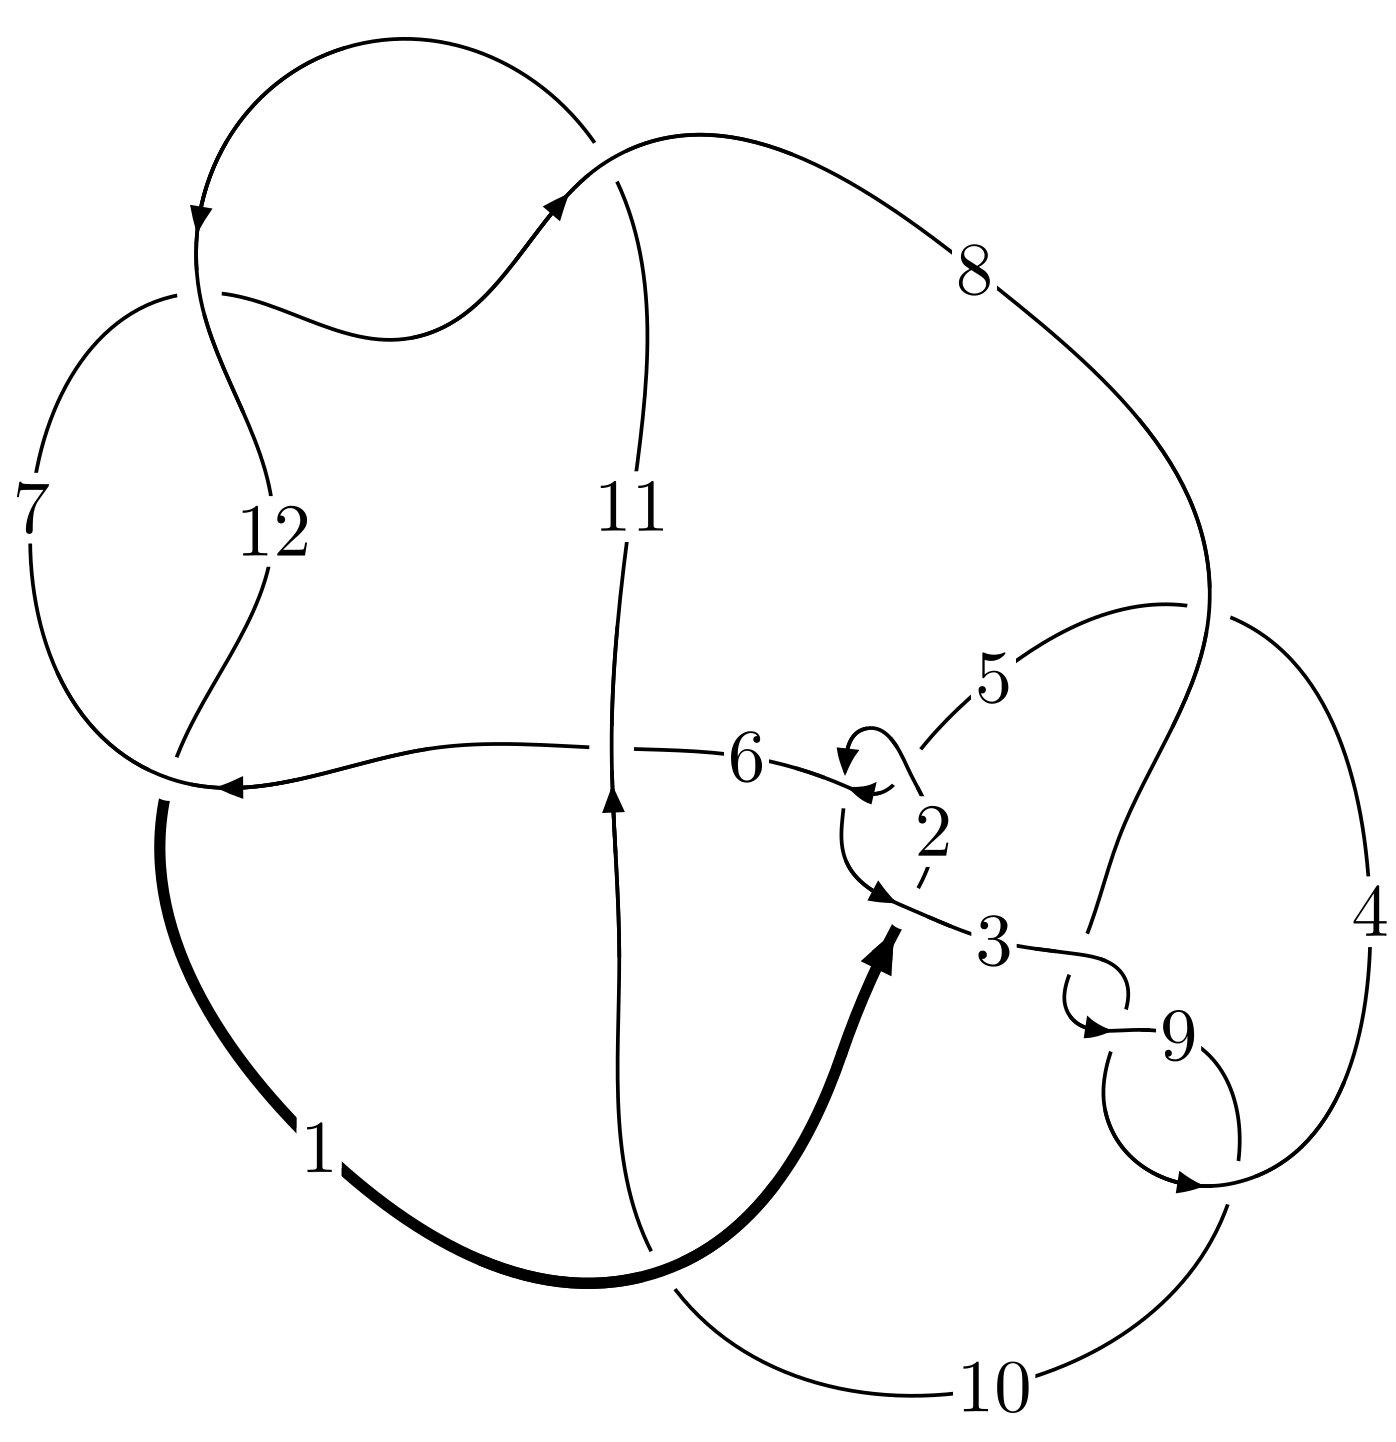
\includegraphics[width=112pt]{../../../GIT/diagram.site/Diagrams/png/2559_12n_0470.png}\\
\ \ \ A knot diagram\footnotemark}&
\allowdisplaybreaks
\textbf{Linearized knot diagam} \\
\cline{2-2}
 &
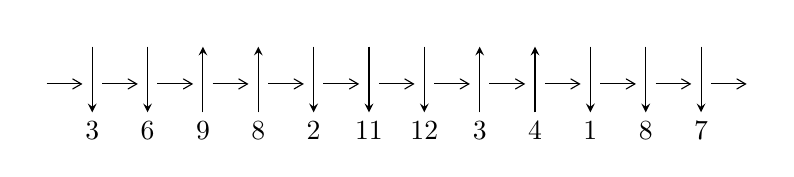
\begin{tikzpicture}[x=20pt, y=17pt]
	% nodes
	\node (C0) at (0, 0) {};
	\node (C1) at (1, 0) {};
	\node (C1U) at (1, +1) {};
	\node (C1D) at (1, -1) {3};

	\node (C2) at (2, 0) {};
	\node (C2U) at (2, +1) {};
	\node (C2D) at (2, -1) {6};

	\node (C3) at (3, 0) {};
	\node (C3U) at (3, +1) {};
	\node (C3D) at (3, -1) {9};

	\node (C4) at (4, 0) {};
	\node (C4U) at (4, +1) {};
	\node (C4D) at (4, -1) {8};

	\node (C5) at (5, 0) {};
	\node (C5U) at (5, +1) {};
	\node (C5D) at (5, -1) {2};

	\node (C6) at (6, 0) {};
	\node (C6U) at (6, +1) {};
	\node (C6D) at (6, -1) {11};

	\node (C7) at (7, 0) {};
	\node (C7U) at (7, +1) {};
	\node (C7D) at (7, -1) {12};

	\node (C8) at (8, 0) {};
	\node (C8U) at (8, +1) {};
	\node (C8D) at (8, -1) {3};

	\node (C9) at (9, 0) {};
	\node (C9U) at (9, +1) {};
	\node (C9D) at (9, -1) {4};

	\node (C10) at (10, 0) {};
	\node (C10U) at (10, +1) {};
	\node (C10D) at (10, -1) {1};

	\node (C11) at (11, 0) {};
	\node (C11U) at (11, +1) {};
	\node (C11D) at (11, -1) {8};

	\node (C12) at (12, 0) {};
	\node (C12U) at (12, +1) {};
	\node (C12D) at (12, -1) {7};
	\node (C13) at (13, 0) {};

	% arrows
	\draw[->,>={angle 60}]
	(C0) edge (C1) (C1) edge (C2) (C2) edge (C3) (C3) edge (C4) (C4) edge (C5) (C5) edge (C6) (C6) edge (C7) (C7) edge (C8) (C8) edge (C9) (C9) edge (C10) (C10) edge (C11) (C11) edge (C12) (C12) edge (C13) ;	\draw[->,>=stealth]
	(C1U) edge (C1D) (C2U) edge (C2D) (C3D) edge (C3U) (C4D) edge (C4U) (C5U) edge (C5D) (C6U) edge (C6D) (C7U) edge (C7D) (C8D) edge (C8U) (C9D) edge (C9U) (C10U) edge (C10D) (C11U) edge (C11D) (C12U) edge (C12D) ;
	\end{tikzpicture} \\
\hhline{~~} \\& 
\textbf{Solving Sequence} \\ \cline{2-2} 
 &
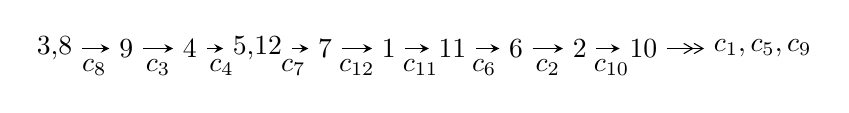
\begin{tikzpicture}[x=23pt, y=7pt]
	% node
	\node (A0) at (-1/8, 0) {3,8};
	\node (A1) at (1, 0) {9};
	\node (A2) at (2, 0) {4};
	\node (A3) at (49/16, 0) {5,12};
	\node (A4) at (33/8, 0) {7};
	\node (A5) at (41/8, 0) {1};
	\node (A6) at (49/8, 0) {11};
	\node (A7) at (57/8, 0) {6};
	\node (A8) at (65/8, 0) {2};
	\node (A9) at (73/8, 0) {10};
	\node (C1) at (1/2, -1) {$c_{8}$};
	\node (C2) at (3/2, -1) {$c_{3}$};
	\node (C3) at (5/2, -1) {$c_{4}$};
	\node (C4) at (29/8, -1) {$c_{7}$};
	\node (C5) at (37/8, -1) {$c_{12}$};
	\node (C6) at (45/8, -1) {$c_{11}$};
	\node (C7) at (53/8, -1) {$c_{6}$};
	\node (C8) at (61/8, -1) {$c_{2}$};
	\node (C9) at (69/8, -1) {$c_{10}$};
	\node (A10) at (11, 0) {$c_{1},c_{5},c_{9}$};

	% edge
	\draw[->,>=stealth]	
	(A0) edge (A1) (A1) edge (A2) (A2) edge (A3) (A3) edge (A4) (A4) edge (A5) (A5) edge (A6) (A6) edge (A7) (A7) edge (A8) (A8) edge (A9) ;
	\draw[->>,>={angle 60}]	
	(A9) edge (A10);
\end{tikzpicture} \\ 

\end{tabular} \\

\footnotetext{
The image of knot diagram is generated by the software ``\textbf{Draw programme}" developed by Andrew Bartholomew(\url{http://www.layer8.co.uk/maths/draw/index.htm\#Running-draw}), where we modified some parts for our purpose(\url{https://github.com/CATsTAILs/LinksPainter}).
}\phantom \\ \newline 
\centering \textbf{Ideals for irreducible components\footnotemark of $X_{\text{par}}$} 
 
\begin{align*}
I^u_{1}&=\langle 
-8.56090\times10^{18} u^{28}+1.26946\times10^{19} u^{27}+\cdots+3.30205\times10^{19} b-1.17890\times10^{20},\\
\phantom{I^u_{1}}&\phantom{= \langle  }4.24911\times10^{17} u^{28}+8.00391\times10^{17} u^{27}+\cdots+6.60410\times10^{19} a-1.61646\times10^{20},\;u^{29}- u^{28}+\cdots+8 u+8\rangle \\
I^u_{2}&=\langle 
-8 a^2 u-6 a^2-10 a u+23 b+4 a-4 u+20,\;4 a^3+2 a^2 u+8 a^2-2 a u+12 a-5 u+6,\;u^2-2\rangle \\
\\
I^v_{1}&=\langle 
a,\;v^2+b+v-1,\;v^3- v+1\rangle \\
\end{align*}
\raggedright * 3 irreducible components of $\dim_{\mathbb{C}}=0$, with total 38 representations.\\
\footnotetext{All coefficients of polynomials are rational numbers. But the coefficients are sometimes approximated in decimal forms when there is not enough margin.}
\newpage
\renewcommand{\arraystretch}{1}
\centering \section*{I. $I^u_{1}= \langle -8.56\times10^{18} u^{28}+1.27\times10^{19} u^{27}+\cdots+3.30\times10^{19} b-1.18\times10^{20},\;4.25\times10^{17} u^{28}+8.00\times10^{17} u^{27}+\cdots+6.60\times10^{19} a-1.62\times10^{20},\;u^{29}- u^{28}+\cdots+8 u+8 \rangle$}
\flushleft \textbf{(i) Arc colorings}\\
\begin{tabular}{m{7pt} m{180pt} m{7pt} m{180pt} }
\flushright $a_{3}=$&$\begin{pmatrix}0\\u\end{pmatrix}$ \\
\flushright $a_{8}=$&$\begin{pmatrix}1\\0\end{pmatrix}$ \\
\flushright $a_{9}=$&$\begin{pmatrix}1\\- u^2\end{pmatrix}$ \\
\flushright $a_{4}=$&$\begin{pmatrix}u\\- u^3+u\end{pmatrix}$ \\
\flushright $a_{5}=$&$\begin{pmatrix}- u^3+2 u\\- u^3+u\end{pmatrix}$ \\
\flushright $a_{12}=$&$\begin{pmatrix}-0.00643404 u^{28}-0.0121196 u^{27}+\cdots+4.90122 u+2.44766\\0.259260 u^{28}-0.384445 u^{27}+\cdots-6.62002 u+3.57020\end{pmatrix}$ \\
\flushright $a_{7}=$&$\begin{pmatrix}-0.271117 u^{28}+0.334733 u^{27}+\cdots+9.14412 u-1.45670\\-0.128384 u^{28}+0.179238 u^{27}+\cdots-0.404961 u-0.978316\end{pmatrix}$ \\
\flushright $a_{1}=$&$\begin{pmatrix}-0.236109 u^{28}+0.260834 u^{27}+\cdots+13.1337 u+0.125839\\-0.0574151 u^{28}+0.133423 u^{27}+\cdots+0.0596710 u-3.33291\end{pmatrix}$ \\
\flushright $a_{11}=$&$\begin{pmatrix}0.252826 u^{28}-0.396565 u^{27}+\cdots-1.71880 u+6.01786\\0.259260 u^{28}-0.384445 u^{27}+\cdots-6.62002 u+3.57020\end{pmatrix}$ \\
\flushright $a_{6}=$&$\begin{pmatrix}0.0314186 u^{28}-0.160388 u^{27}+\cdots+8.16809 u+6.71091\\0.154889 u^{28}-0.224315 u^{27}+\cdots-3.21485 u+3.05436\end{pmatrix}$ \\
\flushright $a_{2}=$&$\begin{pmatrix}-0.236109 u^{28}+0.260834 u^{27}+\cdots+13.1337 u+0.125839\\-0.112639 u^{28}+0.196907 u^{27}+\cdots+1.75075 u-3.53071\end{pmatrix}$ \\
\flushright $a_{10}=$&$\begin{pmatrix}- u^2+1\\u^4-2 u^2\end{pmatrix}$\\&\end{tabular}
\flushleft \textbf{(ii) Obstruction class $= -1$}\\~\\
\flushleft \textbf{(iii) Cusp Shapes $= \frac{39228839356043585039}{33020514644217504884} u^{28}-\frac{61355544613566956791}{33020514644217504884} u^{27}+\cdots-\frac{58856639661756517532}{8255128661054376221} u+\frac{225530309149992021474}{8255128661054376221}$}\\~\\
\newpage\renewcommand{\arraystretch}{1}
\flushleft \textbf{(iv) u-Polynomials at the component}\newline \\
\begin{tabular}{m{50pt}|m{274pt}}
Crossings & \hspace{64pt}u-Polynomials at each crossing \\
\hline $$\begin{aligned}c_{1}\end{aligned}$$&$\begin{aligned}
&u^{29}+4 u^{28}+\cdots+107 u+49
\end{aligned}$\\
\hline $$\begin{aligned}c_{2},c_{5}\end{aligned}$$&$\begin{aligned}
&u^{29}+4 u^{28}+\cdots-11 u+7
\end{aligned}$\\
\hline $$\begin{aligned}c_{3},c_{8},c_{9}\end{aligned}$$&$\begin{aligned}
&u^{29}+u^{28}+\cdots+8 u-8
\end{aligned}$\\
\hline $$\begin{aligned}c_{4}\end{aligned}$$&$\begin{aligned}
&u^{29}-3 u^{28}+\cdots-15272 u+10856
\end{aligned}$\\
\hline $$\begin{aligned}c_{6}\end{aligned}$$&$\begin{aligned}
&u^{29}-2 u^{28}+\cdots-1632 u+289
\end{aligned}$\\
\hline $$\begin{aligned}c_{7},c_{11},c_{12}\end{aligned}$$&$\begin{aligned}
&u^{29}+2 u^{28}+\cdots-4 u+1
\end{aligned}$\\
\hline $$\begin{aligned}c_{10}\end{aligned}$$&$\begin{aligned}
&u^{29}-2 u^{28}+\cdots+16 u+1
\end{aligned}$\\
\hline
\end{tabular}\\~\\
\newpage\renewcommand{\arraystretch}{1}
\flushleft \textbf{(v) Riley Polynomials at the component}\newline \\
\begin{tabular}{m{50pt}|m{274pt}}
Crossings & \hspace{64pt}Riley Polynomials at each crossing \\
\hline $$\begin{aligned}c_{1}\end{aligned}$$&$\begin{aligned}
&y^{29}+52 y^{28}+\cdots-12561 y-2401
\end{aligned}$\\
\hline $$\begin{aligned}c_{2},c_{5}\end{aligned}$$&$\begin{aligned}
&y^{29}-4 y^{28}+\cdots+107 y-49
\end{aligned}$\\
\hline $$\begin{aligned}c_{3},c_{8},c_{9}\end{aligned}$$&$\begin{aligned}
&y^{29}-43 y^{28}+\cdots+1344 y-64
\end{aligned}$\\
\hline $$\begin{aligned}c_{4}\end{aligned}$$&$\begin{aligned}
&y^{29}-127 y^{28}+\cdots+3814324416 y-117852736
\end{aligned}$\\
\hline $$\begin{aligned}c_{6}\end{aligned}$$&$\begin{aligned}
&y^{29}+22 y^{28}+\cdots+1534012 y-83521
\end{aligned}$\\
\hline $$\begin{aligned}c_{7},c_{11},c_{12}\end{aligned}$$&$\begin{aligned}
&y^{29}+30 y^{28}+\cdots+28 y-1
\end{aligned}$\\
\hline $$\begin{aligned}c_{10}\end{aligned}$$&$\begin{aligned}
&y^{29}+46 y^{28}+\cdots+124 y-1
\end{aligned}$\\
\hline
\end{tabular}\\~\\
\newpage\flushleft \textbf{(vi) Complex Volumes and Cusp Shapes}
$$\begin{array}{c|c|c}  
\text{Solutions to }I^u_{1}& \I (\text{vol} + \sqrt{-1}CS) & \text{Cusp shape}\\
 \hline 
\begin{aligned}
u &= \phantom{-}0.316769 + 0.789145 I \\
a &= \phantom{-}0.904647 + 0.546825 I \\
b &= \phantom{-}0.08467 - 1.45881 I\end{aligned}
 & \phantom{-}5.67795 + 2.38900 I & \phantom{-}1.37819 - 3.19465 I \\ \hline\begin{aligned}
u &= \phantom{-}0.316769 - 0.789145 I \\
a &= \phantom{-}0.904647 - 0.546825 I \\
b &= \phantom{-}0.08467 + 1.45881 I\end{aligned}
 & \phantom{-}5.67795 - 2.38900 I & \phantom{-}1.37819 + 3.19465 I \\ \hline\begin{aligned}
u &= \phantom{-}1.097700 + 0.412064 I \\
a &= -0.595170 - 0.691055 I \\
b &= -0.599694 + 0.489209 I\end{aligned}
 & \phantom{-}3.55184 + 4.25255 I & -0.45867 - 6.46134 I \\ \hline\begin{aligned}
u &= \phantom{-}1.097700 - 0.412064 I \\
a &= -0.595170 + 0.691055 I \\
b &= -0.599694 - 0.489209 I\end{aligned}
 & \phantom{-}3.55184 - 4.25255 I & -0.45867 + 6.46134 I \\ \hline\begin{aligned}
u &= -1.204910 + 0.143277 I \\
a &= -0.293068 - 0.232714 I \\
b &= -0.549997 + 0.336152 I\end{aligned}
 & \phantom{-}3.28345 - 0.44058 I & \phantom{-0.000000 }      -6
0. 10   - 0.545557 I \\ \hline\begin{aligned}
u &= -1.204910 - 0.143277 I \\
a &= -0.293068 + 0.232714 I \\
b &= -0.549997 - 0.336152 I\end{aligned}
 & \phantom{-}3.28345 + 0.44058 I & \phantom{-0.000000 -}     -6
0. 10   + 0.545557 I \\ \hline\begin{aligned}
u &= -1.160470 + 0.608867 I \\
a &= -1.27126 + 1.44803 I \\
b &= -0.20515 - 1.50770 I\end{aligned}
 & \phantom{-}10.09380 - 7.21117 I & \phantom{-}2.41941 + 5.24025 I \\ \hline\begin{aligned}
u &= -1.160470 - 0.608867 I \\
a &= -1.27126 - 1.44803 I \\
b &= -0.20515 + 1.50770 I\end{aligned}
 & \phantom{-}10.09380 + 7.21117 I & \phantom{-}2.41941 - 5.24025 I \\ \hline\begin{aligned}
u &= -0.505279 + 0.361091 I \\
a &= \phantom{-}2.34984 - 1.72007 I \\
b &= -0.110424 + 1.342560 I\end{aligned}
 & \phantom{-}1.94298 + 1.80277 I & -0.49805 + 1.45271 I \\ \hline\begin{aligned}
u &= -0.505279 - 0.361091 I \\
a &= \phantom{-}2.34984 + 1.72007 I \\
b &= -0.110424 - 1.342560 I\end{aligned}
 & \phantom{-}1.94298 - 1.80277 I & -0.49805 - 1.45271 I\\
 \hline 
 \end{array}$$\newpage$$\begin{array}{c|c|c}  
\text{Solutions to }I^u_{1}& \I (\text{vol} + \sqrt{-1}CS) & \text{Cusp shape}\\
 \hline 
\begin{aligned}
u &= -1.37914\phantom{ +0.000000I} \\
a &= -0.746430\phantom{ +0.000000I} \\
b &= -0.204561\phantom{ +0.000000I}\end{aligned}
 & \phantom{-}3.21988\phantom{ +0.000000I} & \phantom{-}2.48730\phantom{ +0.000000I} \\ \hline\begin{aligned}
u &= \phantom{-}1.43955 + 0.14926 I \\
a &= -0.504031 + 1.268030 I \\
b &= -0.275994 - 1.361500 I\end{aligned}
 & \phantom{-}8.43378 - 2.66043 I & \phantom{-}4.12391 + 2.05291 I \\ \hline\begin{aligned}
u &= \phantom{-}1.43955 - 0.14926 I \\
a &= -0.504031 - 1.268030 I \\
b &= -0.275994 + 1.361500 I\end{aligned}
 & \phantom{-}8.43378 + 2.66043 I & \phantom{-}4.12391 - 2.05291 I \\ \hline\begin{aligned}
u &= -0.114786 + 0.495278 I \\
a &= \phantom{-}0.919138 + 0.026052 I \\
b &= \phantom{-}0.313764 + 0.344047 I\end{aligned}
 & -0.229419 - 1.001340 I & -3.84178 + 6.77489 I \\ \hline\begin{aligned}
u &= -0.114786 - 0.495278 I \\
a &= \phantom{-}0.919138 - 0.026052 I \\
b &= \phantom{-}0.313764 - 0.344047 I\end{aligned}
 & -0.229419 + 1.001340 I & -3.84178 - 6.77489 I \\ \hline\begin{aligned}
u &= \phantom{-}1.47083 + 0.27563 I \\
a &= -1.01428 - 1.86721 I \\
b &= -0.03771 + 1.45349 I\end{aligned}
 & \phantom{-}8.55001 + 0.76591 I & \phantom{-}2.60710 + 0. I\phantom{ +0.000000I} \\ \hline\begin{aligned}
u &= \phantom{-}1.47083 - 0.27563 I \\
a &= -1.01428 + 1.86721 I \\
b &= -0.03771 - 1.45349 I\end{aligned}
 & \phantom{-}8.55001 - 0.76591 I & \phantom{-}2.60710 + 0. I\phantom{ +0.000000I} \\ \hline\begin{aligned}
u &= -0.493739 + 0.068040 I \\
a &= \phantom{-}1.050210 + 0.145523 I \\
b &= \phantom{-}0.245555 + 1.259730 I\end{aligned}
 & \phantom{-}2.00232 - 3.30872 I & \phantom{-}2.94068 + 6.38072 I \\ \hline\begin{aligned}
u &= -0.493739 - 0.068040 I \\
a &= \phantom{-}1.050210 - 0.145523 I \\
b &= \phantom{-}0.245555 - 1.259730 I\end{aligned}
 & \phantom{-}2.00232 + 3.30872 I & \phantom{-}2.94068 - 6.38072 I \\ \hline\begin{aligned}
u &= \phantom{-}0.460911\phantom{ +0.000000I} \\
a &= \phantom{-}1.05971\phantom{ +0.000000I} \\
b &= \phantom{-}0.666711\phantom{ +0.000000I}\end{aligned}
 & -1.88534\phantom{ +0.000000I} & -1.71060\phantom{ +0.000000I}\\
 \hline 
 \end{array}$$\newpage$$\begin{array}{c|c|c}  
\text{Solutions to }I^u_{1}& \I (\text{vol} + \sqrt{-1}CS) & \text{Cusp shape}\\
 \hline 
\begin{aligned}
u &= \phantom{-}0.352362\phantom{ +0.000000I} \\
a &= \phantom{-}2.57874\phantom{ +0.000000I} \\
b &= -0.415198\phantom{ +0.000000I}\end{aligned}
 & -2.30685\phantom{ +0.000000I} & \phantom{-}3.93900\phantom{ +0.000000I} \\ \hline\begin{aligned}
u &= -1.78867 + 0.13031 I \\
a &= \phantom{-}0.165694 - 0.713641 I \\
b &= \phantom{-}0.825140 + 0.480483 I\end{aligned}
 & \phantom{-}13.9627 - 6.7087 I & \phantom{-0.000000 } 0 \\ \hline\begin{aligned}
u &= -1.78867 - 0.13031 I \\
a &= \phantom{-}0.165694 + 0.713641 I \\
b &= \phantom{-}0.825140 - 0.480483 I\end{aligned}
 & \phantom{-}13.9627 + 6.7087 I & \phantom{-0.000000 } 0 \\ \hline\begin{aligned}
u &= \phantom{-}1.80898 + 0.05309 I \\
a &= -0.009185 - 0.570290 I \\
b &= \phantom{-}0.750595 + 0.635424 I\end{aligned}
 & \phantom{-}14.4546 + 1.4510 I & \phantom{-0.000000 } 0 \\ \hline\begin{aligned}
u &= \phantom{-}1.80898 - 0.05309 I \\
a &= -0.009185 + 0.570290 I \\
b &= \phantom{-}0.750595 - 0.635424 I\end{aligned}
 & \phantom{-}14.4546 - 1.4510 I & \phantom{-0.000000 } 0 \\ \hline\begin{aligned}
u &= \phantom{-}1.79922 + 0.20085 I \\
a &= \phantom{-}0.94548 + 1.76730 I \\
b &= \phantom{-}0.30618 - 1.52419 I\end{aligned}
 & -19.0200 + 10.8571 I & \phantom{-0.000000 } 0 \\ \hline\begin{aligned}
u &= \phantom{-}1.79922 - 0.20085 I \\
a &= \phantom{-}0.94548 - 1.76730 I \\
b &= \phantom{-}0.30618 + 1.52419 I\end{aligned}
 & -19.0200 - 10.8571 I & \phantom{-0.000000 } 0 \\ \hline\begin{aligned}
u &= -1.88226 + 0.01785 I \\
a &= \phantom{-}0.40598 - 1.84877 I \\
b &= \phantom{-}0.22960 + 1.57941 I\end{aligned}
 & -17.6742 - 2.1522 I & \phantom{-0.000000 } 0 \\ \hline\begin{aligned}
u &= -1.88226 - 0.01785 I \\
a &= \phantom{-}0.40598 + 1.84877 I \\
b &= \phantom{-}0.22960 - 1.57941 I\end{aligned}
 & -17.6742 + 2.1522 I & \phantom{-0.000000 } 0\\
 \hline 
 \end{array}$$\newpage\newpage\renewcommand{\arraystretch}{1}
\centering \section*{II. $I^u_{2}= \langle -8 a^2 u-6 a^2-10 a u+23 b+4 a-4 u+20,\;4 a^3+2 a^2 u+8 a^2-2 a u+12 a-5 u+6,\;u^2-2 \rangle$}
\flushleft \textbf{(i) Arc colorings}\\
\begin{tabular}{m{7pt} m{180pt} m{7pt} m{180pt} }
\flushright $a_{3}=$&$\begin{pmatrix}0\\u\end{pmatrix}$ \\
\flushright $a_{8}=$&$\begin{pmatrix}1\\0\end{pmatrix}$ \\
\flushright $a_{9}=$&$\begin{pmatrix}1\\-2\end{pmatrix}$ \\
\flushright $a_{4}=$&$\begin{pmatrix}u\\- u\end{pmatrix}$ \\
\flushright $a_{5}=$&$\begin{pmatrix}0\\- u\end{pmatrix}$ \\
\flushright $a_{12}=$&$\begin{pmatrix}a\\0.347826 a^{2} u+0.434783 a u+\cdots-0.173913 a-0.869565\end{pmatrix}$ \\
\flushright $a_{7}=$&$\begin{pmatrix}0.391304 a^{2} u+0.739130 a u+\cdots+1.30435 a+0.521739\\0.0869565 a^{2} u-0.391304 a u+\cdots-1.04348 a-0.217391\end{pmatrix}$ \\
\flushright $a_{1}=$&$\begin{pmatrix}\frac{1}{2} u\\-0.260870 a^{2} u-0.826087 a u+\cdots-0.869565 a-0.347826\end{pmatrix}$ \\
\flushright $a_{11}=$&$\begin{pmatrix}0.347826 a^{2} u+0.434783 a u+\cdots+0.826087 a-0.869565\\0.347826 a^{2} u+0.434783 a u+\cdots-0.173913 a-0.869565\end{pmatrix}$ \\
\flushright $a_{6}=$&$\begin{pmatrix}\frac{1}{2} u\\-0.260870 a^{2} u-0.826087 a u+\cdots-0.869565 a-0.347826\end{pmatrix}$ \\
\flushright $a_{2}=$&$\begin{pmatrix}\frac{1}{2} u\\-0.260870 a^{2} u-0.826087 a u+\cdots-0.869565 a-0.347826\end{pmatrix}$ \\
\flushright $a_{10}=$&$\begin{pmatrix}-1\\0\end{pmatrix}$\\&\end{tabular}
\flushleft \textbf{(ii) Obstruction class $= 1$}\\~\\
\flushleft \textbf{(iii) Cusp Shapes $= -\frac{24}{23} a^2 u-\frac{64}{23} a^2-\frac{76}{23} a u-\frac{80}{23} a-\frac{12}{23} u-\frac{124}{23}$}\\~\\
\newpage\renewcommand{\arraystretch}{1}
\flushleft \textbf{(iv) u-Polynomials at the component}\newline \\
\begin{tabular}{m{50pt}|m{274pt}}
Crossings & \hspace{64pt}u-Polynomials at each crossing \\
\hline $$\begin{aligned}c_{1},c_{5}\end{aligned}$$&$\begin{aligned}
&(u-1)^6
\end{aligned}$\\
\hline $$\begin{aligned}c_{2}\end{aligned}$$&$\begin{aligned}
&(u+1)^6
\end{aligned}$\\
\hline $$\begin{aligned}c_{3},c_{4},c_{8}\\c_{9}\end{aligned}$$&$\begin{aligned}
&(u^2-2)^3
\end{aligned}$\\
\hline $$\begin{aligned}c_{6}\end{aligned}$$&$\begin{aligned}
&(u^3- u^2+1)^2
\end{aligned}$\\
\hline $$\begin{aligned}c_{7}\end{aligned}$$&$\begin{aligned}
&(u^3+u^2+2 u+1)^2
\end{aligned}$\\
\hline $$\begin{aligned}c_{10}\end{aligned}$$&$\begin{aligned}
&(u^3+u^2-1)^2
\end{aligned}$\\
\hline $$\begin{aligned}c_{11},c_{12}\end{aligned}$$&$\begin{aligned}
&(u^3- u^2+2 u-1)^2
\end{aligned}$\\
\hline
\end{tabular}\\~\\
\newpage\renewcommand{\arraystretch}{1}
\flushleft \textbf{(v) Riley Polynomials at the component}\newline \\
\begin{tabular}{m{50pt}|m{274pt}}
Crossings & \hspace{64pt}Riley Polynomials at each crossing \\
\hline $$\begin{aligned}c_{1},c_{2},c_{5}\end{aligned}$$&$\begin{aligned}
&(y-1)^6
\end{aligned}$\\
\hline $$\begin{aligned}c_{3},c_{4},c_{8}\\c_{9}\end{aligned}$$&$\begin{aligned}
&(y-2)^6
\end{aligned}$\\
\hline $$\begin{aligned}c_{6},c_{10}\end{aligned}$$&$\begin{aligned}
&(y^3- y^2+2 y-1)^2
\end{aligned}$\\
\hline $$\begin{aligned}c_{7},c_{11},c_{12}\end{aligned}$$&$\begin{aligned}
&(y^3+3 y^2+2 y-1)^2
\end{aligned}$\\
\hline
\end{tabular}\\~\\
\newpage\flushleft \textbf{(vi) Complex Volumes and Cusp Shapes}
$$\begin{array}{c|c|c}  
\text{Solutions to }I^u_{2}& \I (\text{vol} + \sqrt{-1}CS) & \text{Cusp shape}\\
 \hline 
\begin{aligned}
u &= \phantom{-}1.41421\phantom{ +0.000000I} \\
a &= -1.40536 + 0.78044 I \\
b &= -0.215080 - 1.307140 I\end{aligned}
 & \phantom{-}6.31400 - 2.82812 I & -0.49024 + 2.97945 I \\ \hline\begin{aligned}
u &= \phantom{-}1.41421\phantom{ +0.000000I} \\
a &= -1.40536 - 0.78044 I \\
b &= -0.215080 + 1.307140 I\end{aligned}
 & \phantom{-}6.31400 + 2.82812 I & -0.49024 - 2.97945 I \\ \hline\begin{aligned}
u &= \phantom{-}1.41421\phantom{ +0.000000I} \\
a &= \phantom{-}0.103619\phantom{ +0.000000I} \\
b &= -0.569840\phantom{ +0.000000I}\end{aligned}
 & \phantom{-}2.17641\phantom{ +0.000000I} & -7.01950\phantom{ +0.000000I} \\ \hline\begin{aligned}
u &= -1.41421\phantom{ +0.000000I} \\
a &= -0.963939\phantom{ +0.000000I} \\
b &= -0.569840\phantom{ +0.000000I}\end{aligned}
 & \phantom{-}2.17641\phantom{ +0.000000I} & -7.01950\phantom{ +0.000000I} \\ \hline\begin{aligned}
u &= -1.41421\phantom{ +0.000000I} \\
a &= -0.16448 + 1.83384 I \\
b &= -0.215080 - 1.307140 I\end{aligned}
 & \phantom{-}6.31400 - 2.82812 I & -0.49024 + 2.97945 I \\ \hline\begin{aligned}
u &= -1.41421\phantom{ +0.000000I} \\
a &= -0.16448 - 1.83384 I \\
b &= -0.215080 + 1.307140 I\end{aligned}
 & \phantom{-}6.31400 + 2.82812 I & -0.49024 - 2.97945 I\\
 \hline 
 \end{array}$$\newpage\newpage\renewcommand{\arraystretch}{1}
\centering \section*{III. $I^v_{1}= \langle a,\;v^2+b+v-1,\;v^3- v+1 \rangle$}
\flushleft \textbf{(i) Arc colorings}\\
\begin{tabular}{m{7pt} m{180pt} m{7pt} m{180pt} }
\flushright $a_{3}=$&$\begin{pmatrix}v\\0\end{pmatrix}$ \\
\flushright $a_{8}=$&$\begin{pmatrix}1\\0\end{pmatrix}$ \\
\flushright $a_{9}=$&$\begin{pmatrix}1\\0\end{pmatrix}$ \\
\flushright $a_{4}=$&$\begin{pmatrix}v\\0\end{pmatrix}$ \\
\flushright $a_{5}=$&$\begin{pmatrix}v\\0\end{pmatrix}$ \\
\flushright $a_{12}=$&$\begin{pmatrix}0\\- v^2- v+1\end{pmatrix}$ \\
\flushright $a_{7}=$&$\begin{pmatrix}1\\v+1\end{pmatrix}$ \\
\flushright $a_{1}=$&$\begin{pmatrix}v^2+v-1\\v^2-1\end{pmatrix}$ \\
\flushright $a_{11}=$&$\begin{pmatrix}- v^2- v+1\\- v^2- v+1\end{pmatrix}$ \\
\flushright $a_{6}=$&$\begin{pmatrix}- v^2- v+1\\- v^2+1\end{pmatrix}$ \\
\flushright $a_{2}=$&$\begin{pmatrix}v^2+2 v-1\\v^2-1\end{pmatrix}$ \\
\flushright $a_{10}=$&$\begin{pmatrix}1\\0\end{pmatrix}$\\&\end{tabular}
\flushleft \textbf{(ii) Obstruction class $= 1$}\\~\\
\flushleft \textbf{(iii) Cusp Shapes $= -4 v^2+2 v-6$}\\~\\
\newpage\renewcommand{\arraystretch}{1}
\flushleft \textbf{(iv) u-Polynomials at the component}\newline \\
\begin{tabular}{m{50pt}|m{274pt}}
Crossings & \hspace{64pt}u-Polynomials at each crossing \\
\hline $$\begin{aligned}c_{1},c_{2}\end{aligned}$$&$\begin{aligned}
&(u-1)^3
\end{aligned}$\\
\hline $$\begin{aligned}c_{3},c_{4},c_{8}\\c_{9}\end{aligned}$$&$\begin{aligned}
&u^3
\end{aligned}$\\
\hline $$\begin{aligned}c_{5}\end{aligned}$$&$\begin{aligned}
&(u+1)^3
\end{aligned}$\\
\hline $$\begin{aligned}c_{6},c_{10}\end{aligned}$$&$\begin{aligned}
&u^3+u^2-1
\end{aligned}$\\
\hline $$\begin{aligned}c_{7}\end{aligned}$$&$\begin{aligned}
&u^3- u^2+2 u-1
\end{aligned}$\\
\hline $$\begin{aligned}c_{11},c_{12}\end{aligned}$$&$\begin{aligned}
&u^3+u^2+2 u+1
\end{aligned}$\\
\hline
\end{tabular}\\~\\
\newpage\renewcommand{\arraystretch}{1}
\flushleft \textbf{(v) Riley Polynomials at the component}\newline \\
\begin{tabular}{m{50pt}|m{274pt}}
Crossings & \hspace{64pt}Riley Polynomials at each crossing \\
\hline $$\begin{aligned}c_{1},c_{2},c_{5}\end{aligned}$$&$\begin{aligned}
&(y-1)^3
\end{aligned}$\\
\hline $$\begin{aligned}c_{3},c_{4},c_{8}\\c_{9}\end{aligned}$$&$\begin{aligned}
&y^3
\end{aligned}$\\
\hline $$\begin{aligned}c_{6},c_{10}\end{aligned}$$&$\begin{aligned}
&y^3- y^2+2 y-1
\end{aligned}$\\
\hline $$\begin{aligned}c_{7},c_{11},c_{12}\end{aligned}$$&$\begin{aligned}
&y^3+3 y^2+2 y-1
\end{aligned}$\\
\hline
\end{tabular}\\~\\
\newpage\flushleft \textbf{(vi) Complex Volumes and Cusp Shapes}
$$\begin{array}{c|c|c}  
\text{Solutions to }I^v_{1}& \I (\text{vol} + \sqrt{-1}CS) & \text{Cusp shape}\\
 \hline 
\begin{aligned}
v &= \phantom{-}0.662359 + 0.562280 I \\
a &= \phantom{-0.000000 } 0 \\
b &= \phantom{-}0.215080 - 1.307140 I\end{aligned}
 & \phantom{-}1.37919 + 2.82812 I & -5.16553 - 1.85489 I \\ \hline\begin{aligned}
v &= \phantom{-}0.662359 - 0.562280 I \\
a &= \phantom{-0.000000 } 0 \\
b &= \phantom{-}0.215080 + 1.307140 I\end{aligned}
 & \phantom{-}1.37919 - 2.82812 I & -5.16553 + 1.85489 I \\ \hline\begin{aligned}
v &= -1.32472\phantom{ +0.000000I} \\
a &= \phantom{-0.000000 } 0 \\
b &= \phantom{-}0.569840\phantom{ +0.000000I}\end{aligned}
 & -2.75839\phantom{ +0.000000I} & -15.6690\phantom{ +0.000000I}\\
 \hline 
 \end{array}$$\newpage
\newpage\renewcommand{\arraystretch}{1}
\centering \section*{ IV. u-Polynomials}
\begin{tabular}{m{50pt}|m{274pt}}
Crossings & \hspace{64pt}u-Polynomials at each crossing \\
\hline $$\begin{aligned}c_{1}\end{aligned}$$&$\begin{aligned}
&((u-1)^9)(u^{29}+4 u^{28}+\cdots+107 u+49)
\end{aligned}$\\
\hline $$\begin{aligned}c_{2}\end{aligned}$$&$\begin{aligned}
&((u-1)^3)(u+1)^6(u^{29}+4 u^{28}+\cdots-11 u+7)
\end{aligned}$\\
\hline $$\begin{aligned}c_{3},c_{8},c_{9}\end{aligned}$$&$\begin{aligned}
&u^3(u^2-2)^3(u^{29}+u^{28}+\cdots+8 u-8)
\end{aligned}$\\
\hline $$\begin{aligned}c_{4}\end{aligned}$$&$\begin{aligned}
&u^3(u^2-2)^3(u^{29}-3 u^{28}+\cdots-15272 u+10856)
\end{aligned}$\\
\hline $$\begin{aligned}c_{5}\end{aligned}$$&$\begin{aligned}
&((u-1)^6)(u+1)^3(u^{29}+4 u^{28}+\cdots-11 u+7)
\end{aligned}$\\
\hline $$\begin{aligned}c_{6}\end{aligned}$$&$\begin{aligned}
&((u^3- u^2+1)^2)(u^3+u^2-1)(u^{29}-2 u^{28}+\cdots-1632 u+289)
\end{aligned}$\\
\hline $$\begin{aligned}c_{7}\end{aligned}$$&$\begin{aligned}
&(u^3- u^2+2 u-1)(u^3+u^2+2 u+1)^2(u^{29}+2 u^{28}+\cdots-4 u+1)
\end{aligned}$\\
\hline $$\begin{aligned}c_{10}\end{aligned}$$&$\begin{aligned}
&((u^3+u^2-1)^3)(u^{29}-2 u^{28}+\cdots+16 u+1)
\end{aligned}$\\
\hline $$\begin{aligned}c_{11},c_{12}\end{aligned}$$&$\begin{aligned}
&((u^3- u^2+2 u-1)^2)(u^3+u^2+2 u+1)(u^{29}+2 u^{28}+\cdots-4 u+1)
\end{aligned}$\\
\hline
\end{tabular}\newpage\renewcommand{\arraystretch}{1}
\centering \section*{ V. Riley Polynomials}
\begin{tabular}{m{50pt}|m{274pt}}
Crossings & \hspace{64pt}Riley Polynomials at each crossing \\
\hline $$\begin{aligned}c_{1}\end{aligned}$$&$\begin{aligned}
&((y-1)^9)(y^{29}+52 y^{28}+\cdots-12561 y-2401)
\end{aligned}$\\
\hline $$\begin{aligned}c_{2},c_{5}\end{aligned}$$&$\begin{aligned}
&((y-1)^9)(y^{29}-4 y^{28}+\cdots+107 y-49)
\end{aligned}$\\
\hline $$\begin{aligned}c_{3},c_{8},c_{9}\end{aligned}$$&$\begin{aligned}
&y^3(y-2)^6(y^{29}-43 y^{28}+\cdots+1344 y-64)
\end{aligned}$\\
\hline $$\begin{aligned}c_{4}\end{aligned}$$&$\begin{aligned}
&y^3(y-2)^6(y^{29}-127 y^{28}+\cdots+3.81432\times10^{9} y-1.17853\times10^{8})
\end{aligned}$\\
\hline $$\begin{aligned}c_{6}\end{aligned}$$&$\begin{aligned}
&((y^3- y^2+2 y-1)^3)(y^{29}+22 y^{28}+\cdots+1534012 y-83521)
\end{aligned}$\\
\hline $$\begin{aligned}c_{7},c_{11},c_{12}\end{aligned}$$&$\begin{aligned}
&((y^3+3 y^2+2 y-1)^3)(y^{29}+30 y^{28}+\cdots+28 y-1)
\end{aligned}$\\
\hline $$\begin{aligned}c_{10}\end{aligned}$$&$\begin{aligned}
&((y^3- y^2+2 y-1)^3)(y^{29}+46 y^{28}+\cdots+124 y-1)
\end{aligned}$\\
\hline
\end{tabular}
\vskip 2pc
\end{document}